\label{sec:chap5}
\section{簡介}
在上一章中,我們探討了如何使用聲學組型進行非監督式語意檢索。但另一方面,我們觀察到使用聲學組型時的問題:由於聲學組型在訓練時是採用非監督式方法的,因此訓練時系統並無法知道聲音對應到的文字是什麼,導致在分群時無法知道同音的字的意思是什麼,進而使得聲學組型在訓練時會盡量將同樣發音的字群組在一起。以上所述狀況會使檢索結果變差許多,因為同一個聲學組型事實上是對應到很多不同的字,舉其中一個聲學組型為例,其中包含了「網、王、亡、望、往」等字。因此本章試圖解決聲學組型的模糊性,比如說如果能將「網、王、亡、望、往」分為「網」、「王」、「亡」、「望」、「往」等五群,即可大幅地提升檢索系統的成效了。

在此我們使用了其於遞迴式類神經網路語言模型 (Recurrent Neural Network Language Model)~\cite{mikolov2010recurrent, mikolov2011extensions, mikolov2012context} 之詞表示法 (Word Representation),此一詞表示法可以將每一個詞或字表示為一固定長度的向量,並被認為能有效地表示詞或字在句法 (Syntactic)
和語意上的相似度~\cite{mikolov2013linguistic}。由於同一個聲學組型中包含了許多實際上含義不同的字,因此我們的目的是將聲學組型表示為詞表示法,並基於詞表示法為這些聲學組型做分群,以期在句法和詞義的基礎上將原本同音的聲學組型分為不同的聲學組型。


\section{基於遞迴式類神經網路語言模型之詞表示法}

\subsection{基於遞迴式類神經語言模型之詞表示法}
傳統的詞表示法通常將字表示為 1-of-N 編碼,即每個詞都被表示成一個辭典大小的陣列,只有那個詞對應到的維度是一,其它都是零。這種詞表示法的缺點是將每個詞都視為獨立的詞,即詞與詞之間是無相關性的。舉例來說,如果辭典中有「Hotel」、「Hostel」兩個字。1-of-N 編碼會將這兩個字表示為:

\[
   hotel = [1\ 0\ 0\ 0\ 0\ 0\ 0\ 0\ 0\ 0\ 0\ 0\ 0\ 0\ 0\ 0\ 0] \\ 
\]
\[
   hostel = [0\ 0\ 1\ 0\ 0\ 0\ 0\ 0\ 0\ 0\ 0\ 0\ 0\ 0\ 0\ 0\ 0]
\]

於是「Hotel」與「Hostel」兩字的詞表示法取內積後為零,但這是不合理的狀況,因為這兩個字有很強烈的語意關係,因此就有人提出了使用連續空間的詞表示法 (Continuous Space Word Representation)~\cite{collobert2008unified, turian2010word}
,此一方法的目的是用一個高維度的實數陣列代表一個詞,並且當兩個詞在句法上和含義上相近的時候會讓兩個詞表示法很接近。類神經網路語言模型的一個特色是它們將字表示成高維度的實數陣列,而這些詞表示法甚至可以用在許多自然語言處理的工作上。基於遞迴式類神經網路語言模型的詞表示法是目前被廣泛使用的詞表示法之一~\cite{mikolov2010recurrent},模型中的 $\mathcal{U}$ 是一個 $\mathcal{H} \times \mathcal{L}$ 的矩陣,其中 $\mathcal{H}$ 是隱藏層的維度,$\mathcal{L}$則是辭典的長度,而 $\mathcal{U}$
中的每一欄都代表一個詞的詞表示法。雖然類神經網路語言模型在訓練時完全沒有句法(Syntax)、構詞(Morphology)、或語意(Semantics)相關的資訊,但很令人驚訝地,靠著沿時間反向傳遞演算法的最佳化就能夠非常好地在句法和語意上描述這些詞表示法~\cite{mikolov2013linguistic}。

\begin{figure}
\centering
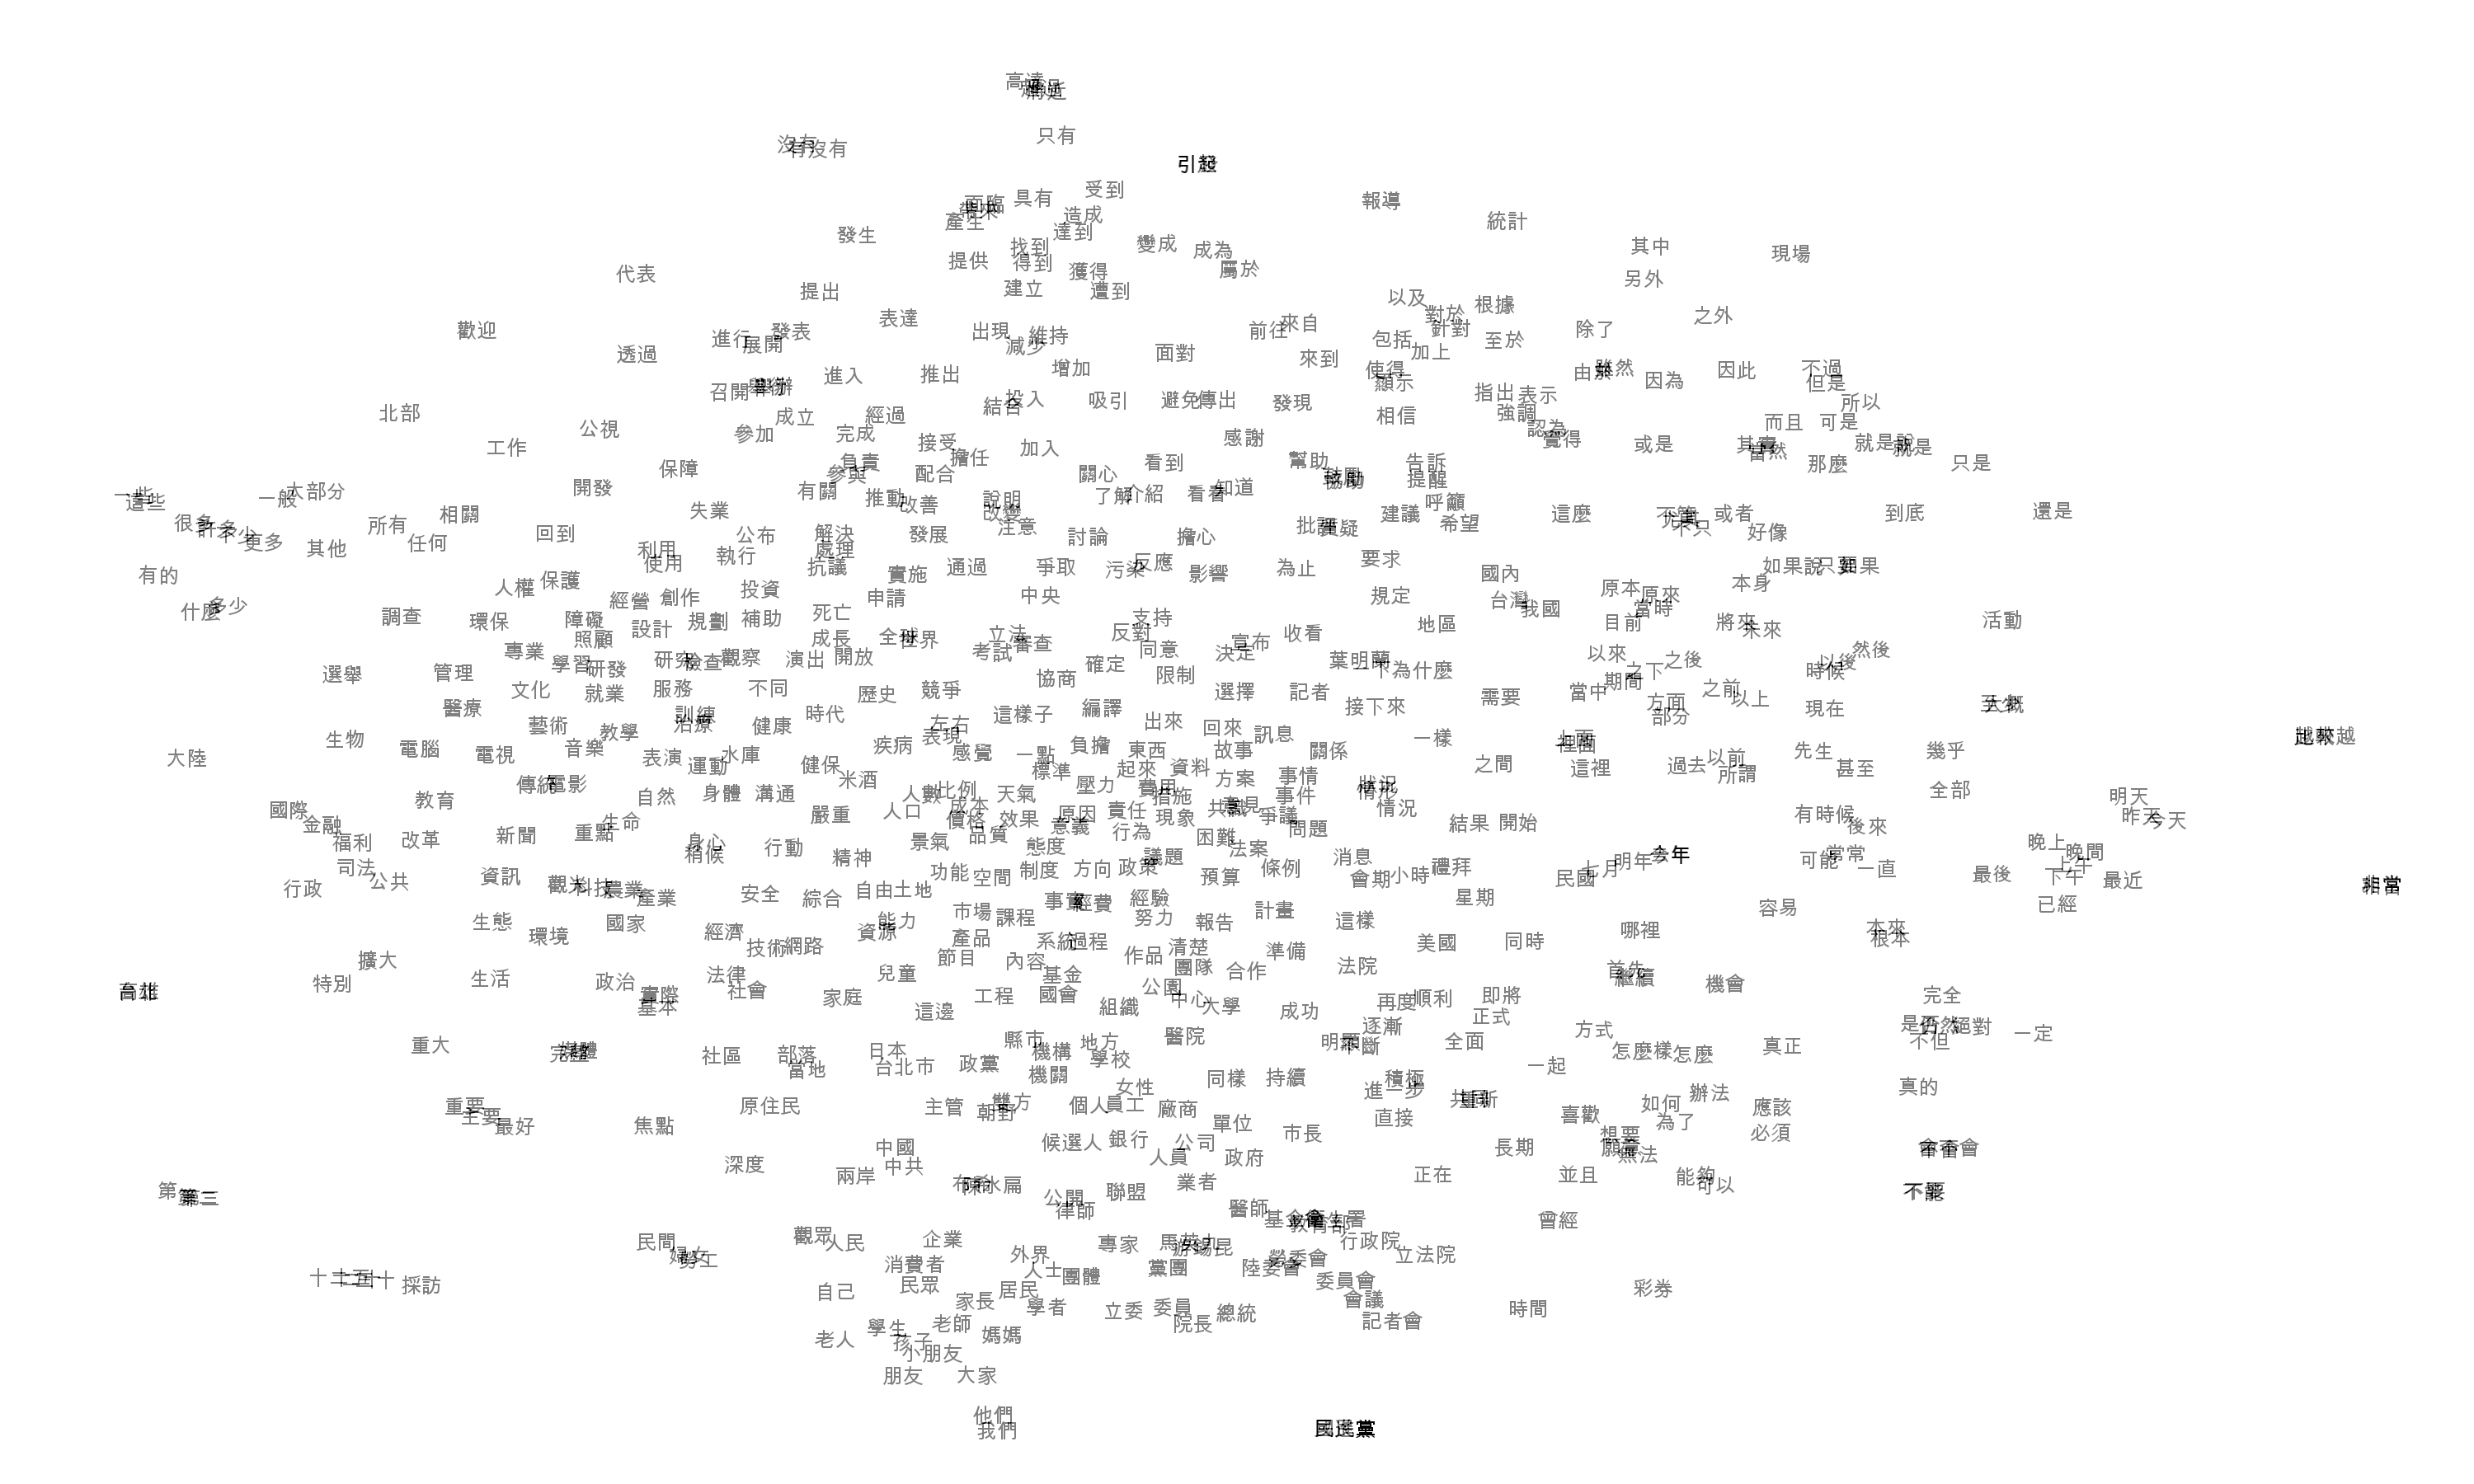
\includegraphics[scale=0.15]{images/chap5_word_rep.png}
\caption{基於遞迴式類神經網路語言模型之詞表示法示意圖} \label{fig:chap5_word_rep}
\end{figure}

圖 ~\ref{fig:chap5_word_rep}
中示意了基於遞迴式類神經網路語言模型之詞表示法,這是使用了公視新聞訓練的詞表示法,隱藏層維度為$100$,並將這些$100$維的詞表示法降為兩維後畫在圖上,由圖中可以看出詞表示法表示詞的能力:如在圖中右方,「今天」、「明天、「昨天」,「晚上」、「晚間」、「上午」、「下午」都被畫在很接近的位置,而這些詞都是用來表示時間的詞彙,又例如圖中下方的「布希」、「陳水扁」被畫得非常接近,而這是由於在這些語料錄製的年份,這兩個人分別是美國與台灣的總統,由這些例子可以看出,雖然遞迴式類神經網路語言模型之詞表示法訓練的過程中是沒有任何關於語意的知識的,但是它卻可以很好地捕捉到詞彙在語意上的資訊,因此很適合用在自然語言處理。

\section{以詞表示法改善非監督式語意檢索}
\label{sec:chap5_algorithm}
演算法之示意如圖 ~\ref{fig:chap5_system},圖上方的紫色框框中為訓練資料,其中的每一行代表一句由聲學組型組合而成的句子,由於其中每一個聲學組型實際上都可能代表了很多不同的詞或字,因此我們在每一次的迴圈當中要對一個聲學組型進行分群。我們的做法是在每一個迴圈中選定一個聲學組型進行分群,如圖 ~\ref{fig:chap5_system} 中的迴圈中選定了 $p_1$ 這個聲學組型,並將所有的 $p_1$ 視為是不同的聲學組型,如 $p_{1\_1},
p_{1\_2}, p_{1\_3}, ...$,並進行K平均分群演算法 (K-Means Clustering) 基於這些詞和字的詞表示法進行分群,由於這些詞表示法攜有了許多的句法和詞義的資訊,因此這個分群的結果會將這些聲學組型按照句法和語意分開,以期在進行K平均分群後,每一群中包含的聲學組型對應到的中文詞彙會盡量一致。

\begin{figure}
\centering
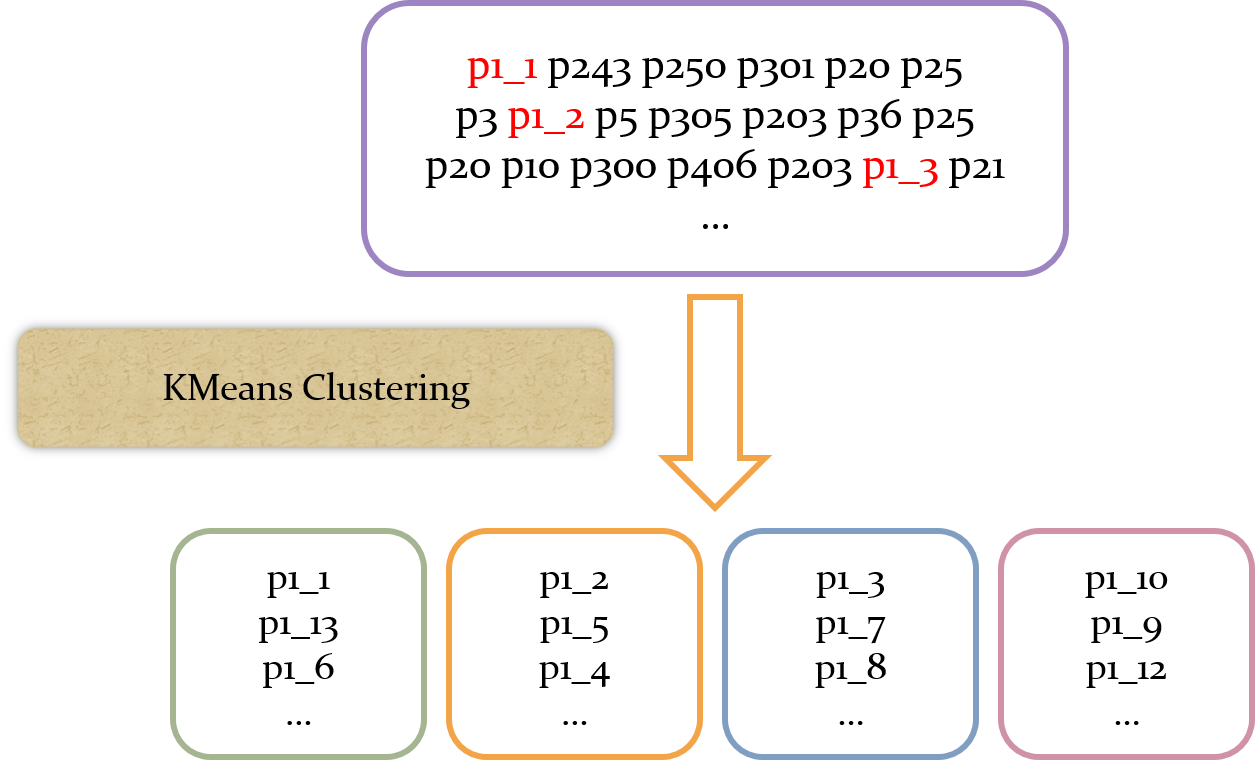
\includegraphics[scale=0.6]{images/chap5_system.png}
\caption{演算法示意圖} \label{fig:chap5_system}
\end{figure}

演算法的步驟為在每個迴圈都從所有的聲學組型中選一個聲學組型(選過的不再選),稱為 $p$,並在這個迴圈中重複以下的步驟:

1. 將訓練語料中所有的$p$都視為不同的聲學組型,亦即將所有的$p$按照出現順序改為$p_1, p_2, p_3...$。

2. 將修改後的訓練語料做為遞迴式類神經網路語言模型的訓練語料,並訓練一套遞迴式類神經網路語言模型。

3. 取出遞迴式類神經網路語言模型的$\mathcal{U}$做為所有聲學組型的詞表示法,並用K平均分群法將這些詞表示法分為K群,這K群的聲學組型即為不同的聲學組型,標示為$p_{k1}, p_{k2}, p_{k3}, ...$。


\section{實驗基礎架構}
本章實驗所使用的設定同 ~\ref{sec:chap4_exp_setup},使用的語料為2001年間從電台廣播中錄下的4小時新聞,並手動切成5034篇語音文件,每篇語音文件大約包含了$1至3$句的語句。用來辨識的語言模型是用1999年間收集的新聞文章 (包含4000萬個詞彙)
訓練而成,辭典中包含了62000個詞彙,聲學模型是用2000年間收集的8小時廣播新聞訓練而成的音節內(Intra-syllable) 右方資訊相依(Right-context-dependent) 聲韻母模型 (Initial-Final Models)。辨識後的唯一最佳序列的字元正確率為 (Character Accuracy) 為75.27\%。
本章中使用的聲學組型設定為將 5034 句的新聞語音文件辨識成 208 個字單位的語音組型。
總共測試了30組口語查詢詞,這些口語查詢詞都使用了 ~\ref{sec:chap4_decode_query} 轉為對應的聲學組型查詢詞,每組查詢詞都有人工標注對應的相關文件,而這些相關文件中「一定要」包含查詢詞。

\section{實驗結果}
實驗結果如圖 ~\ref{fig:chap5_result1} 和 ~\ref{fig:chap5_result2} 所示。橫軸為迴圈的次數,每次迴圈都從中找出一個聲學組型進行 ~\ref{sec:chap5_algorithm} 的演算法,由於總共有208個聲學組型,因此橫軸到208後即為對所有的聲學組型都執行一次演算法。縱軸為檢索結果的平均準確率,紅線為檢索系統的基準 (Baseline) 檢索結果,同 ~\ref{fig:chap4_resulta} 中的紅線,為使用動態時間扭曲產生的第一次檢索結果。 

\begin{figure}
\centering
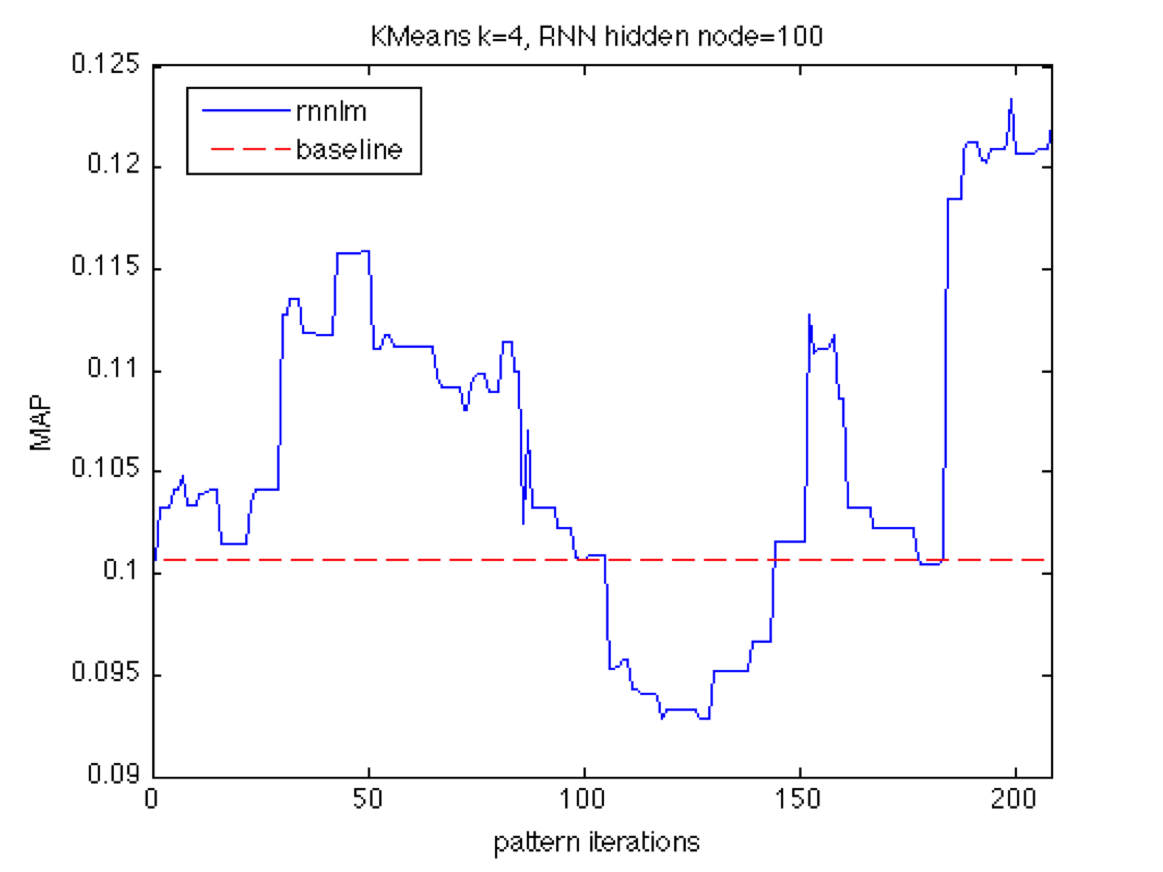
\includegraphics[scale=0.5]{images/chap5_result1.png}
\caption{實驗結果:K分群法的K設定為4,潛藏層長度設為100} \label{fig:chap5_result1}
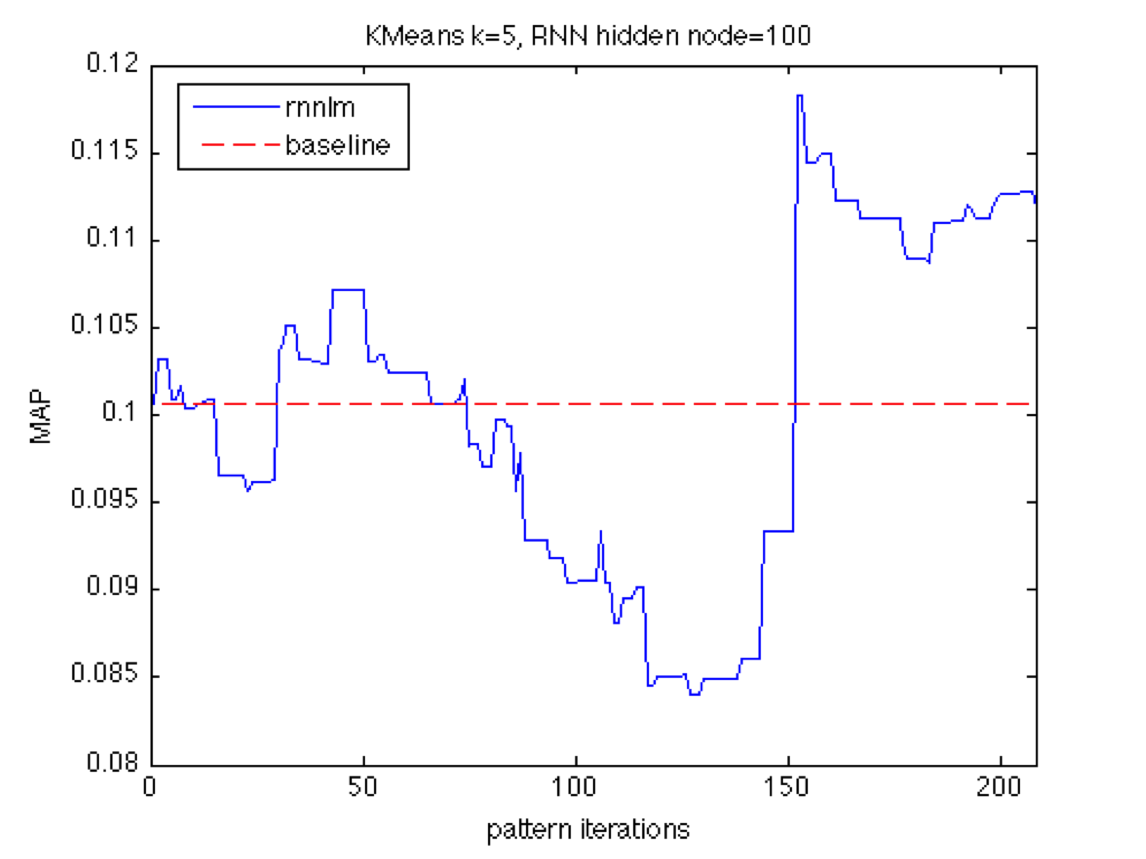
\includegraphics[scale=0.5]{images/chap5_result2.png}
\caption{實驗結果:K分群法的K設定為5,潛藏層長度設為100} \label{fig:chap5_result2}
\end{figure}

由圖中可以觀察到,在大部分的時間點,此方法都能使檢索的成效增加,在最高點的平均準確率可以到達$12.23\%$,進步量相對於基準檢索結果為$21.4\%$,證明此方法確實能有效地將同音的聲學組型切為對檢索結果更有貢獻的聲學組型,並給予聲學組型更多地語意資訊,但此方法的缺點目前的強健性 (Robustness) 還不夠,無法讓平均準確率在所有的迴圈中都穩定上升,但能夠讓某些聲學組型有很大幅的成長。未來可能的改進方向如下:

1. 嘗試用不同的分群演算法,並使用開發語料 (Development Set) 調整分群演算法的參數。

2. 觀察為何有些聲學組型能獲得大幅的進步,並試圖找出判斷依據,如此一來就可以只分會獲得進步的聲學組型,並不要對會退步的聲學組型做這套演算法。

\section{本章總結}
本章試圖解決聲學組型在訓練時只考慮同音的問題,並試圖為聲學組型加入更多的句法與語意資訊,再將加入額外資訊的聲學組型應用於語音文件檢索系統中,並獲致了初步的進步。
